%\documentclass[conference,draftcls]{IEEEtran}
\documentclass[conference,final]{IEEEtran}
%\documentclass[conference,manuscript]{IEEEtran}

%\usepackage{setspace}
%\onehalfspacing

%\usepackage{ifpdf}
\usepackage[utf8]{inputenc}
\usepackage{cite}
\usepackage{paralist}
%\usepackage[pdftex]{graphicx}
\usepackage[dvips]{graphicx} 
%\usepackage{pslatex}
\usepackage{caption}
\usepackage{subcaption}
%\graphicspath{{.}{images/}} 
%\DeclareGraphicsExtensions{.eps}
\usepackage[cmex10]{amsmath}
%\usepackage{url}
%\usepackage[rgb]{xcolor}
%\usepackage{pdfcomment}

%\usepackage[tight,footnotesize]{subfigure}
%\usepackage[caption=false]{caption}
%\usepackage[font=footnotesize]{subfig}
%\usepackage[caption=false,font=footnotesize]{subfig}
%\usepackage{fixltx2e}
%\usepackage{stfloats}
%
%\usepackage[rgb]{xcolor}
%\usepackage{pdfcomment}

%\newcommand{\dme}[2]{\pdfmarkupcomment[markup=Highlight,color=yellow]{#1}{#2}}
%\newcommand{\notedme}[1]{\raisebox{0pt}[0pt][0pt]{\pdfcomment[open=true,color=blue]{#1}}}
%\newcommand{\todo}[1]{\pdfmarkupcomment[markup=Highlight,color=red]{#1}{todo}}

% \newcommand{\red}[1]{\pdfmarkupcomment[markup=Highlight,color=red]{#1}}
% \newcommand{\green}[1]{\pdfmarkupcomment[markup=Highlight,color=green]{#1}}
% \newcommand{\grey}[1]{\pdfmarkupcomment[markup=Highlight,color=gray]{#1}}
\newcommand*{\bd}[1]{\multicolumn{1}{|c|}{\bfseries #1}}


% correct bad hyphenation here
\hyphenation{op-tical net-works semi-conduc-tor}


\begin{document}
\title{Helping Secure Robots in WSN Environments by Monitoring WSN Software Updates for Intrusions}
%\title{Securing Robotics in WSN Integrated Environment: Intrusion Detection of WSN Software Update}

\author{
		\IEEEauthorblockN{	A S M Ashraful Alam, David Eyers, Zhiyi Huang 	}
	\IEEEauthorblockA{Department of Computer Science, University of Otago, New Zealand, Email: \{aalam, dme, hzy\}@cs.otago.ac.nz} 
}


% use for special paper notices
%\IEEEspecialpapernotice{(Invited Paper)}

\maketitle

%\doublespacing
\begin{abstract}
Robotics and  Wireless Sensor Network (WSN) collaboration is an emerging research field in which both technologies can benefit from integrated implementations.
A robot operating in WSN assisted environments can dynamically push instructions using over the air (OTA) update protocols to alter sensors to suit the requirements.
In this paper, an Intrusion Detection System (IDS) for a WSN  software update protocol is designed and simulated. 
When the protocol modifies the running software in a mote, the mote sends related  information to the WSN sink. 
The IDS analyses the update phenomena of each of the motes in the network and computes an Intrusion Warning Score (IWS) that indicates a possible intrusion due to an illegitimate software update.
%\notedme{Mentioning robots more than just in the first word would be good}
\end{abstract}


%\begin{keyword}
%Wireless Sensors, WSN, Intrusion Detection System, IDS, Security
%\end{keyword}


%ICARA does accept papers on sensors. With collaborative robotics increasing rapidly, security of inter-robot communication over wireless media is of great importance. Your proposed paper would be of interest to ICARA attendees and we look forward to receiving your paper by 27th October.

\section{Introduction}
\label{sec:intro}

Wireless Sensor Networks (WSN) have attracted robotics
researchers because of problems they can potentially solve, such as
robot localisation, path finding, sensing, and mapping. 
%
Integrated
WSNs and robotics applications augment a robot's capabilities for decision-making.
% interaction potential and decision making capabilities.
% and services where WSNs can be deployed in the environment. 
% <dme> I don't understand the above
Mission critical robotics applications in military, mining, team collaboration, or applications such as companionship
for the elderly can employ wireless sensors as well. Conversely,
robotics can also be utilised to solve WSN problems like
sensor deployment or relocation in hostile environments; assisting data aggregation; and acting as data mules~\cite{Shue13}.
WSNs can greatly enhance
the perception capabilities of robots and provide infrastructure
for robust inter-robot communication. Mobile robot navigation is another emerging research area where robotics and
wireless sensors collaborate. Multiple robots can benefit from
navigating in WSN-assisted environments without depending
on GPS signals. Robots can also dynamically change the
sensor applications over the air (OTA) to suit changes
in environmental sensing requirements. However, the security of
WSN technologies is a major concern.

Wireless sensor devices in WSNs are known as nodes or
motes. The manager node, which is generally connected to
a workstation and a long lasting power source is called a sink
or a base station. All sensor nodes in a WSN have a unique
identification number---the \emph{Node ID}. Intrusions during software
updates primarily indicate uploading inappropriate software
that perform undesired actions, having replacing the
sensor operating system (OS) software. We use the term `update time'
to denote when any mote begins executing a new version
of the software image. Data exchange in WSN takes place
locally using a neighbourhood discovery process, following
an autonomous relay mechanism that does not require a routing table.

WSNs often need to be updated after deployment to accommodate bug-fixes, changes in requirements, or alterations to
the environment~\cite{ISI:000253439700120}.
%sensing applications, or scientific requirements
% <dme> unclear intellectual structure of that list: messy overlaps between scientific requirements and requirements, for example.
Certain protocols, such as Deluge, can solve this problem
by facilitating OTA updates. Deluge is an efficient and reliable protocol.
It addresses several network programming issues, e.g., dealing
with program objects larger than the sensor memory, and working in environments with high packet loss rates, variable node density
and asymmetric links~\cite{1031506, 1127826}.
%Deluge is an interesting protocol
%to investigate any phenomena related to OTA reprogramming.
% <dme> above doesn't add anything. It doesn't say why it's interesting.

Software update in WSNs is a tricky process that has
effects beyond the software updates themselves. 
The mote must reboot the OS to the new application.
During
this time, security measures on the sensor motes are deactivated or
unavailable for a short period of time. Additionally, the update
process across the whole WSN contributes to a significant
increase in traffic that an adversary may exploit to mask his
actions. An attacker can target this time to clandestinely initiate
an illegitimate update and inject his own program image
to serve his intended purpose. This enables an adversary to
steal sensitive information, log network events, even effect complete
denial of service.

Implementation of security techniques in WSNs are critical
and challenging because of constrained resources in the sensor motes.
Moreover, capability of devices that can compromise security
computationally grows at enormous speed in comparison to
sensors. 
%
%In addition to that,
WSNs have special vulnerabilities
that do not exist in wired networks. Wireless channels are
inherently considered to be less secure. Secure protocols
like WPS, PKM and likewise are inappropriate in WSNs.
% <dme> needs citations ideally: you've not said what these are
Reliability and safety critics, and other researchers, have
frequently pointed out that security issues in WSNs have not
been sufficiently addressed, and that WSNs are not yet secure
enough for deployment within mission critical applications like
robotics.

In contrast to the problems described above, the relatively
simple communication protocols and the design of WSNs
makes it easy to perform some types of intrusion detection within them~\cite{quing09}.
An Intrusion Detection System (IDS) does not prevent an attacker, but it can detect break-in events and raise alerts. It
may also be able to report the location and extent of the break-in. 
In this paper we present an algorithm, which considers a
centralised approach to detect the intrusion in the case of a WSN
software update. The algorithm requires a minor modification
of the OTA update protocol to send back a datagram packet
containing the update time~\cite{tep116}.
%\notedme{broken approach? (i.e. Skipping from simulation to IDS implementation when that's not possible.)}

The information carried by the
datagram is processed and analysed to work out an
%`Surprise Score' 
% <dme> quoted term introduced but used nowhere else in document.
Intrusion Warning Score (IWS) to indicate a
possible intrusion. 
This work's contributions are two fold: 
\begin{inparaenum}
\item  The IDS identifies anomalies in software update patterns
and scores them quantitatively;
\item It is demonstrated that the IDS
can indicate the location of an intrusion point and the possible extent
of intrusion.
%scheme i.e., the IDS expectations can provide useful insight for designing secure WSN.
\end{inparaenum}


%\subsection{Organisation of the paper }
The rest of this paper is structured in the following way. 
In Section~\ref{sec:lit},  
%this paper is structured in the following way.
%In Section II, 
we provide an overview of our findings from
intrusion related research works in WSN. We seek software
update security aspects not addressed by the present WSN
security research and the reasons behind this.  
In Section~\ref{sec:meth}, we describe a brief overview of the system design and the experiment methodology. Then we present the findings from the
experiments, analyse the result and present our evaluation in
Section~\ref{sec:eval}.  
Finally, we conclude our arguments in Section~\ref{sec:concl}.

\section{Research in WSN Intrusion Detection}
\label{sec:lit}

%The following section describes the earlier research effort
%in the field and relates it to motivation of the study.

The software update process using OTA protocols is vulnerable
in existing networks due to a lack of cryptographic protections in sensor motes. 
Software update is also a lucrative target in order to effect widespread attacks.
%and a lucrative attack target for several reasons. 
% First,
% the ability to infect a software update process implies effects
% beyond the updates itself. Secondly, cryptographic protection in
% sensors is inadequate. Constrained computational capacity and
% resources make it possible to compromise the cryptographic
% measures incorporated in the implemented WSN OSs~\cite{aes2011}.
% <dme> the above should have been fixed. It doesn't make sense, and isn't correct in as much as I think I know what you mean. Just because it was in the review copy doesn't mean it should stay wrong in the camera-ready.
A  malicious intruder can replicate as an authentic
image source and advertise a new program version that the
other motes cannot repudiate.
%
% Thirdly, there is no mechanism to check the integrity of the entire
% image object, because it is infeasible when the size of the object exceeds
% the size of available sensor memory.
% %\notedme{Interesting argument! I like it. Although it could be that _most_ of the pages get integrity-checked, and Deluge does use pages...}
% Fourthly, even if an OTA update protocol incorporates on-chip hardware based encryption,
% cryptography alone cannot prevent all attacks. 
%\notedme{Weak point. No evidence is provided, and no examples given.}
% <dme> the above points are too weak for publication, I think. You could form hash trees to fix point 3, and 4 doesn't have any evidence or context provided.
Techniques of
different types of attacks on WSNs have been described by~\cite{DBLP:journals/corr/abs-1301-3022}. 
% <dme> don't use publications as nouns. Say by "blah et al.~\cite{...}"
Countermeasures against these attacks are computationally
expensive and energy intensive---employing them exposes
the WSN to some other kinds of attacks, such as DoS through
resource exhaustion.
% <dme> above point isn't strong: sending packets does the same sort of thing, and comms is the problem, not computing.
Once an attacker has compromised a node, they can utilise the knowledge that they gain
%Fifthly, an attacker can extract valuable
%information about the network from a physically compromised
%node. He can utilise the knowledge 
to initiate Sybil attacks~\cite{syb02}.
%, even
%can replace the nodes with the illegitimate and malicious ones,
%which can imitate a legal update process. 
Considering the above, some researchers suggest a complete redesign
of security mechanisms in WSNs~\cite{quing09}.


The OTA update protocols may act as carriers of malicious
code in the network. For example, Deluge achieves reliability
using a density-aware epidemic property that 
%works on a state
%machine principle 
% <dme> the above is meaningless in isolation. Turing machines are state machines too...
follows a few local rules to achieve global
behaviour~\cite{1031506}.
It follows that breach at any one point weakens
the whole WSN. An attacker may pretend to be an authentic
source and disappear after successful introduction of the illegitimate image to one mote in the network. 
Because of the epidemic propagation property in Deluge, this illegitimate image will spread over the entire network.
% OTA protocol security mechanisms, which are cryptographic, would be unable to
% detect the breach and would allow the network to be flooded
% by the malicious application~\cite{Karlof:2004:TLL:1031495.1031515}.
% <dme> no idea what the above means.
In recent years, researchers
have suggested several intrusion or anomaly detection means
to secure WSN, alongside the other cryptographic approaches.
The cryptographic approaches employed in resource constrained sensors do not guarantee a secure operating environment.
An attacker with superior abilities is able to compromise the sensors. 
Thus it is useful to employ some other security measures, for
example: an IDS. Purpose of an IDS is to detect suspicious
behaviour in the network, and to provides useful information about
intrusion.
%\marginnote{Ease of attacking OTA protocol}[2cm]

%%%%I WANT TO CHANGE THIS PORTION
The proposed IDS techniques vary greatly in their ideas and approaches.
Rule-based misuse detection  techniques identify undesired activities based  on abnormality signature.
They aim to detect known attacks.
However, they are ineffective against previously unknown attacks.
Additionally, they may wrongly identify legitimate activities as intrusion because of similarity with the signature~\cite{372146, 1515559, ISI:000298891500099, Chen:2009:NMI:1516241.1516282, 1424814, Strikos_afull}.
A decentralised, hierarchical, rule-based IDS follows a network-based approach  and monitors exchanged  messages to detect intrusion. 
The technique relies on hierarchical routing  and monitors the cluster heads to trace messages~\cite{ioa07}.
However, rule-based hierarchical routing method does not guarantee using the best energy path.
%}ISI:000298891500099, Chen:2009:NMI:1516241.1516282, 1424814, Strikos_afull}. %Rule-based, node-based traffic
They also are often ineffective against novel attacks and may wrongly identify legitimate activities as intrusion because of similarities with a malicious signature. 
The other rule-based IDSs also are often ineffective against new attacks and may wrongly identify legitimate activities as intrusion because of similarities with a malicious signature. 
In response to this difficulty, anomaly based IDSs build signatures based on defined normal activity.
They use statistical probability and significance to identify anomalies. Unfortunately, a system may display previously unknown behaviour.
For example: rare critical events like earthquakes or tsunamis may raise false positive intrusion alert in sensors employed for other environmental monitoring.
On the other hand, an intrusion that masks its pattern under the hood of normal behaviour, for example: increased packet traffic during OTA update, would go undetected~\cite{ISI:000257882502160, 1593102, 1290173, ngai07}. %4024996
The techniques described above use different kinds of machine learning tools, such as support vector machines.
In contrast, specification-based and reputation-based techniques rely on manual input for defining normal and anomalous behaviour with lesser reliance on automation.
The techniques are inherently slow and not effective against previously unknown attack techniques.
However, these techniques also have not been proved to be very effective because human interaction are more prone to errors and require more learning time~\cite{Chen:2009:NMI:1516241.1516282, 4085803, Ko2001}. 


Approaches to the design of IDS mechanisms %are either distributed or centrally controlled. They 
employ techniques like key management, encryption and authentication to protect services like localisation, data aggregation, cluster formation, and time synchronisation.
%It is considered that 
The goal is to protect specific services against specific attacks e.g, forwarding, sinkhole, and wormholes, under certain conditions~\cite{1639675, 6096939, sink08, 5172466}.
%Although approaches described above
Despite innovative ideas, only a few IDSs are able to address the security issues related to software updates in WSNs.
Hence, we propose an analytical tool that is passive in nature and can provide valuable insight into the propagation characteristics of OTA reprogramming protocol. 
The technique has been tested on Deluge.
We have exploited services from standard protocols to gather timing information from motes in  the WSN and then process the timing information for intrusion detection.
Use of timing analysis approach is a novel technique in IDS for WSN.
The IDS identifies anomaly in software update pattern in terms of quantitative score. 
A higher score indicates a higher probability of intrusion at some point in the WSN~\cite{aalam14, auspdc15}. 
The IDS  gathers processed information from the sensors, is centrally controlled and resides outside the WSN.
The external placement of IDS has obvious advantage of utilising minimum amount of vital sensor resources, such as energy, for processes related to arriving at decision about some potential intrusion event.

% While timing analysis mechanism is non-existent in the WSN, some of the IDSs use traffic analysis or packet inspection  techniques.
% It can be argued that traffic analysis approach is potentially comparable to proposed timing analysis.
% The argument can be quite intense because traffic analysis considers both throughput and latency, and latency is essentially about timing.
% <dme> the above makes little sense to me.

Use of a quantitative measure such as the IWS to identify intruders is not new in WSN security research.
A cooperative distributed IDS for mobile Ad-hoc networks (MANET) detects intrusion based on a quantitative measure of packet forwarding percentage~\cite{hua03}.
The experimental results are based on simulations in NS-2.\footnote{NS-2 is an open-source real-time network simulation tool that can be used to define different scenario}
The technique can be applied to resource constraint MANETs.
However, requirement of very high magnitudes of data processing turns this technique into one impractical for employment in resource constrained sensors environment. 
An algorithm for detecting the intruder in sinkhole attacks identifies the intruder through analysing the network flow information and uses a mathematical function for this purpose.  According to this technique, the suspected node has a  function  value greater than the threshold function value.
For the data from this node, it is also noticeably inconsistent with other nodes in the area~\cite{ngai07}. 
The authors claim to evaluate the performance of the proposed algorithm through simulations, but they have not presented any details of the simulation environment or framework.
Moreover, in the simulation the sensors adopted IEEE 802.11 standard compliant MAC protocol, which is used for Wi-Fi networks and not WSNs.
It is worth mentioning that WSNs are typically compliant with the IEEE 802.15.4 standard, which was defined four years before the publication~\cite{893287}.
However, the systems referred above use quantitative measures to compare against some threshold value to decide on  the possibility of an intrusion.
The techniques are quite different in their usage from the approach we have presented where the measure of quantitative score or the IWS additionally indicates possibility or severity of an intrusion.
The quantitative calculation that we have presented is very simple. 
In our view, any computation task employed in WSN needs to be simple and computationally lightweight.
Otherwise, there is a risk that the scheme is so energy expensive that the detection system will not be deployable in practice.
%expected to cut down upon  so much of energy resources that the scheme will render the detection system to be practically unemployable.


Onat and Miri~\cite{1512911} present an IDS design that considers a statistical treatment similar to the one we proposed, yet the techniques have subtle differences.
Their IDS deals with node impersonation and resource depletion attacks only.
In this approach, each node builds an expectation of the statistics of received packets based on the last $N$ packets received from each neighbour.
If packets received from any neighbour display anomalous patterns after a predefined number of consecutive packets, intrusion alarms may be raised.
Unfortunately, the  packet count statistics are not suitable in the OTA software update scenario.
There is a significant increase in packet traffic owing to software update process itself. 
This puts the mechanism off balance.
However, the mechanism of statistical treatment on information over a time period motivates us to employ timing analysis approach on the context of OTA update protocol.


\section{Methodology}
\label{sec:meth}
In this section, we give an overview of the system design and the simulation environment used in our evaluation. % and procedures.
%The original system design is quite elaborate, but details have been left out to accommodate the space limitation.
% <dme> I don't understand why you think it's elaborate. It's actually really simple!
%It's helpful to both writer and reader to organise this section chronologically: that is, describe each procedure in the order it was performed. For example, DNA-extraction, purification, amplification, assay, detection. Or, study area, study population, sampling technique, variables studied, analysis method.
%The proposed IDS will be evaluated using a set of simulations. %in comprehensive simulations.
%While the system has been elaborately designed and aimed at testbed evaluation, it has not yet been performed at this stage of the research. 
%\notedme{Dropped sentence here. What does ``aimed at testbed evaluation'' mean?}
% <Ashraf>> I meant evaluation using a testbed implementation
%The testbed implementation will be evaluated at some point in the future.

%\notedme{You should redefine the term IWS in the body text I think. My rule of thumb is that you introduce abbreviations independently in the abstract and in the body text. Of course if you don't use an abbreviation subsequently, you shouldn't introduce it.}
%The raw data generated from simulation logs were processed, related and  analysed to produce the IWS.
%<Ashraf>>That is done now



\subsection*{System Overview}
\label{subsec:sysdeg}
The IDS resides on a computing system that is physically connected to the sink.
%The system  relies on existing protocols for its operations.
% <dme> ! (a new abbreviation for me---approximately "Why are you saying this? Isn't it obvious?")
Information necessary for IDS operations are collected utilising standard transport layer protocols. 
The IDS analyses the update time of  each of the motes in the WSN and computes the IWS using our proposed Equation~\ref{eqn2}---
% and indicates the cases of a possible intrusion, i.e., a probable illegitimate update.
%The IWS, update time and image version information can be utilised to indicate location and extent of intrusion---

\begin{equation}
\label{eqn2} 
	\mathit{IWS} = \sum \limits_{i=0}^{n} \frac{\left| \mu_i - t_i \right|}{\sigma_i + 1}
\end{equation}
where, 
\begin{inparaenum}
\item $\mathit{i}$---mote index;%\notedme{Why were you using capital letters all through here?} 
\item $\mathit{t_i}$---image update time at mote $\mathit{i}$;  
\item $\mathit{\mu_i}$---mean update time at mote $\mathit{i}$;  
\item $\mathit{\sigma_i}$---standard deviation of update time at mote $\mathit{i}$. 
\end{inparaenum}

The intrusion detection algorithm requires some modification of the update protocol to enable an automatic reporting service in the mote by using a datagram packets to carry latest update information to the sink.
The collection of update information can follow realistic mechanisms such as using Active Message technique\cite{tep116} or using the Collection Tree Protocol~\cite{tep123, ctptosn2014}.
All motes in the WSN are assumed to have time synchronisation accurate to 1~$\mu$s, e.g., achieved using the Time Synchronized Mesh Protocol~\cite{Pister08tsmp:time}.
% devices e.g., motes stay synchronised to each other} protocol 
% <dme> !
The timing information carried by the datagram is therefore synchronised with other nodes in the WSN and can be used readily for processing by the IDS.

\begin{figure}[btp]
    \centering
	\resizebox{\linewidth}{!}{
	    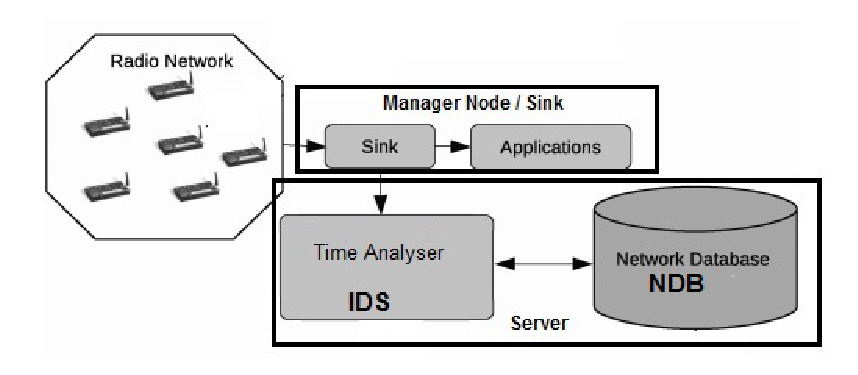
\includegraphics[width=\linewidth]{IDS_fw}	
	}
    \caption{IDS Framework}
    \label{fig:ids_fw}
\end{figure}

\subsubsection*{IDS Framework}
\label{ssc:ids_fw}

The IDS framework components and chronology of the activities associated with the IDS have been shown in Figure~\ref{fig:ids_fw}.
The IDS has three types of components:
\begin{inparaenum}
\item the motes in the WSN radio network that are subject to legitimate or illegitimate update e.g., intrusion attempt; 
\item an IDS transport client (ITC) application that runs on the sink and works in coordination with the IDS to assists in intrusion detection; and
%The sink is protected from all kinds of security breaches whether it is physical or logical. 
\item an IDS application that runs on a system with higher computing resources e.g., a server, which is physically attached to the sink, and houses a network database (NDB).
\end{inparaenum}

%%% <ashraf> strike out
%\begin{inparaenum}
%\item Updates are initiated using Deluge protocol;
%\item Deluge disseminates the new software image using the motes en route to reach all the motes using a relay mechanism; 
%\item The nodes deliver their timing information to the sink using an AM packet;
%\item AM packets from the distant nodes rely on the other nodes en route to reach the sink using a relay mechanism; and
%\item The ITC application in the sink delivers revelent information to the IDS for processing. 
%\end{inparaenum}
%The IDS analyses the acquired timing information to arrive at decision.
\begin{figure}[btp]
    \centering
	\resizebox{\linewidth}{!}{
	    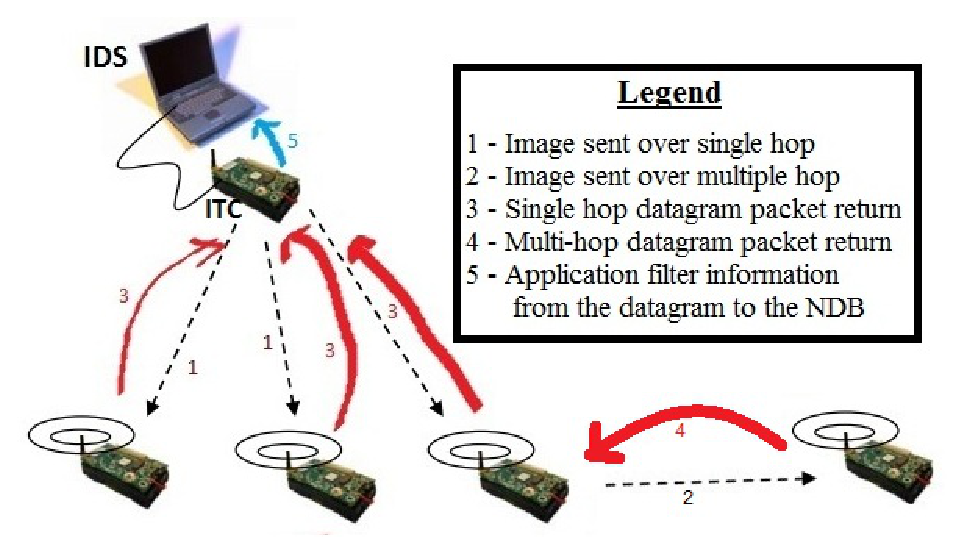
\includegraphics[width=\linewidth]{IDS}
	}    
    \caption{IDS Modelling}
    \label{fig:ids_model}
\end{figure}

\subsubsection*{Gathering Timing Information}
\label{ssc:ga_info}
%% <ashraf> We cannot go into these details in this paper; space limitation
The intrusion detection activity begins when a software update takes place.
The motes perform their part by endorsing update time, software version, mote ID  and initiating a datagram to the sink. 
%An AM packet initiated for the IDS has several fields: destination address, type identifier that indicates the update time information and the protocol for IDS, timing information and a checksum value.
%[DO WE WANT TO INCLUDE THE PATH TAGGING; MAY BE LATER - IT INCREASES RELIABILITY, NOT DIRECTLY $IDS$ ACTIVITY?]
%[path tagging is good, but in all cases, what's the risk from intruders messing with the reported data?]
%[PATH TAGGING CAN BE USED AS HEART-BEAT MESSAGE]
The packet travels to the sink using a synchronous acknowledgement mechanism in transport layer protocols~\cite{tep116}.
%When it arrives at the sink, the checksum value is examined by the ITC to ensure that the packet content has not been altered en route.
After checking for correctness of the datagram contents, the ITC then inserts the update time, mote ID and related information to the NDB in the IDS.
The IDS maintains an identifier to differentiate among different update times from different runs for the same mote.
%
%The first software update run in the WSN is considered to be legitimate and the IDS takes this timing information as baseline.
%It is possible and desirable that the IDS is trained with several other update runs.
%More training improved the ability of the IDS to detect intrusion more accurately.
%Utilising multiple runs are useful and beneficial as it increases accuracy and dependency.
%However, the IDS needs to be manually controlled to enable multiple training runs.
%Outcome from these runs are statistically treated to build the baseline.

\subsubsection*{Identifying Intrusion}
\label{ssc:cal_iws} 
The IDS builds anomaly signatures or baseline data from authenticated initial software update runs. % are considered to be 
The subsequent updates are subject to verification against these signatures.
The time analyser module in the IDS inspects the NDB once an update activity has been detected.
It determines the changes in the statistics of the update time and calculates IWS based on utility function in Equation~\ref{eqn2}. IWS indicates the possibility of an intrusion. If the IWS is high enough to be considered an intrusion, the IDS sorts the timing data for that run and identifies the source of intrusion as the mote reporting from the lowest update time.
The IDS also identifies the extent of intrusion from mote ID and version information in the database.



%
%\subsubsection*{Building Intrusion Warning Zone}
%\label{ssc:iw_zone}
%The IDS can build a scale of possible expected range of IWS for a topology and can classify the IWS in different zones to imply certain warning levels.
%While reporting severity or likelihood of an intrusion in quantitative term like the IWS is useful, it is more beneficial if the quantity is associated with some kind of interpretation.
%The technique of associating such interpretation has been established by identifying Intrusion Warning Zone (IWZ) from a scale built from maximum expected IWS in a topology.
%We have used a heuristic trial and error method to build the IWZ.
%Threshold for building of Intrusion Warning Zone (IWZ) depends on the assumed ability of the IDS having IWS knowledge of all possible intrusions in the network.
%%\notedme{This is not clear: you're jumping to talking about thresholds before describing what they are or why you want them.}
%Such knowledge can be built by replicating intrusion activity from all nodes in the network.
%In situations where it is not possible, replicating intrusion activity from the furthest few nodes may serve the purpose.
%The heuristics follows from statistical techniques and feasibility of finding easily identifiable boundary.
%%%<Ashraf>> I need to work more on this, I agree.
%The IDS considers an IWS up to 10\% from the scale to be safe and marks as `GREEN' zone, an IWS above 30\% to be possible intrusion and is marked as `RED' zone.
%%\notedme{Why? Where's the science here?}
%However, an IWS within the range of 10\%---30\% can neither be considered safe, nor an intrusion, hence is marked as `GREY' to indicate a situation where rules are not known.
%However, the thresholds are not conclusive and may require some variation based on the density, power level used in the WSN and scale of deployment.
%%\notedme{This does not read strongly. It sounds like you're trying to make too much out of this: just state that for convenience of discussion, you define these zones. They seem entirely subjective to me: useful for discussion, but no more than that.}

\subsection*{Threat Model}
%What are the security aspects it does not handle?
%Why does not it handle them?

%\notedme{This is a start, but it's not very clearly written. Talking about the expected capabilities of attackers and vulnerabilities of the system would be good.}
The threat model is directed towards injection of unauthorised program images to infect the entire WSN.
The IDS is expected to handle malicious node update, node compromise, and node failure.
In addition to this, the IDS also considers a threat model where a new node pops up and injects the new software image by compromising existing WSN security mechanism.
%The main threat scenario that the IDS is expected to handle is compromise of a particular node in the WSN and then attacker being able to utilise the same node or replicate the node to inject a new software image using Deluge protocol in the WSN.
%However, once the new image transfer has been injected, the node may remain alive or disappear.
%In case the compromised mote disappears, WSN would consider it as a node failure instead of node compromise.

%We assume that an  attacker  can take over one or more nodes deployed in hostile environment, and can access the code in a compromised node. 
We assume that the nodes are physically protected and not accessible by the attacker.
The only way an intruder can launch an attack is through the wireless network.
An attacker can also use cryptanalysis to represent a false identity without physically compromising a node.
We also assume that the sensors are equipped with a protected memory area that cannot be overwritten by the OTA update process.
The protected area can only be programmed physically through a sensor programming board and needs to follow specific security routines that are beyond the scope of this paper.
The update protocol and other security codes are housed in this protected memory area.
This implies that the update protocol cannot be compromised by the intruder. 
%He is able to access the code in a compromised node by employing superior computing power. 
%However, he has  no special  access to  the  network and 
% <dme> they have plenty of special access to the network??
%However, he is unable to modify the underlying protocols running in the uncompromised nodes.

The paper assumes several WSN settings and capabilities.
One of the most important assumptions is that there is a single  sink. 
It further assumes that the sink is protected from all kinds of attacks and cannot be compromised. 
The system does not consider mote mobility scenarios and assumes a static WSN.


\subsection*{Experimental Settings}
\label{subsec:sim_env}

The IDS requires Deluge to report the time when it begins  executing  a new version of some software.
The Deluge protocol was originally implemented in TinyOS and later has been ported to other embedded operating systems including Contiki.\footnote{http://www.contiki-os.org}
We used Deluge protocol implemented in Contiki v2.7 on a system running on Ubuntu 12.04.
%[So this will eventually need citation and a self-contained description.]
`Cooja',\footnote{https://github.com/contiki-os/contiki/wiki/An-Introduction-to-Cooja} a network simulator for Contiki, was used to simulate the software update pattern associated with Deluge protocol.
%\notedme{Best to give academic citations, or footnote URLs for these technologies.}
%We also used a plugin for Contiki called Mobility to aid our experiential setup.
%Although the plugin was designed to deal with positions over time for the nodes in the simulation, we used it to load the exact location of the sensor motes into the `Cooja' simulator. 

%\subsection*{Design of Experiments}
%\label{subsec:exp_des}

The simulation environment allows the software update pattern to be observed, by detecting when each WSN node completes the software update.
% reporting the time at which the new software update completes and starts executing.
The simulations evaluated the proposed IDS in different WSN topologies and explored the effect of parameters like power level.
%\notedme{Compare the commented and rewritten sentences here. Terms like `cautiously' are not useful unless the context is clear.} %<Ashraf>> Thanks
Evaluating the IDS on each of the topologies consisted of several test runs.
The test runs were of two kinds: 
\begin{inparaenum}
\item test runs aimed at establishing baseline data consisted of 20 individual simulations initiated from the sink; and
\item simulations that replicated intrusion initiated at different nodes except the sink.
\end{inparaenum}
The results from these simulations were used to model the expected pattern for a particular topology.
%
%\subsection*{Topologies}
%\label{subsec:topos}
The topologies were designed to observe the performance and effectiveness %of the  that were established using number of trial and error test runs 
of the proposed system in different environmental scenarios. 
In addition to this, effects of changes in parameters like power level on the IDS behaviour were also observed.
%\notedme{Not clear what you're talking about, specifically.}
We used topologies in experiments that had many shapes such as: linear, circular, elliptical, double rings, wide line, grid, tree and other random topologies, but do not have space to describe all of them here.
%The names of the topologies here indicate that in each case the motes were deployed along the circumference of the geometrical shape that enabled packet propagation to take place according to a designed fashion.\notedme(1){drop---too obvious to justify saying.}
%In each topology, minimum 20 nodes were deployed for a test to take place. 
%More motes were necessary to replicate certain topologies.
% Table~\ref{tab:topos} shows the number of motes used in experiments in corresponding topological  deployments.
%The motes were placed at a distance of 30--35m to allow  multiple transmission paths to all motes. % <dme> en-dash for number ranges, not em-dash	% <ashraf> I am trying to increase my English and LaTeX vocabulary
%The radio transmission power level was set at 100\% which has an approximate maximum effective transmission range of 50m, potentially interfering with motes up to 100m away.
% <dme> why is the node spacing relevant to the work presented? I've assumed not and removed it for now...


\subsection*{Procedure}
\label{subsec:proc}
%
%Experiment procedure  was a combination of activities such as running simulation, analysing system log and processing data to arrive at a conclusion. 
%\notedme{I'd just list the three steps if there are only three steps. Too simple to be worth using text to introduce subsequent short blocks of text.}
%
%
%\subsubsection*{Processing  of Individual Test Run}
%\label{ssc:test_runs}
%Step 1: Running simulation
\subsubsection*{Step 1} 
In the environmental arrangement described above, all motes in the WSN were booted up at same time running one version of a diagnostic application. 
The diagnostic application would necessarily report its time, version number and mote ID on the serial terminal every second at its serial port. 


%Step 2: Stopping the simulation
\subsubsection*{Step 2} 
The sink dynamically began the update process and propagated another version of the software image using the Deluge protocol. %, which is also called 
Whenever the transfer to a mote was complete, the new image would replace the old one and reboot to begin executing itself.
The  new application also causes the motes to report their time, version number and mote ID on the serial terminal. 
In a real system, the suggested modified Deluge protocol that runs with the OS would report the information to the sink using a datagram.
The simulator continued until all the motes in the WSN were updated and the reported events were logged. 
%Step 3: Filtering out mote update time and distance
%The update time of each mote were filtered out  and were sorted in ascending order of update time.
% <dme> no need to state the obvious

%Step 4: Calculating the euclidean distance and sorting
%A cpp application was used to take input from this semi-processed information and another file that preserved the position information of the motes in the deployment.
%The application processed the data to find out the euclidean distance of the motes from the sink.
%It additionally sorted the rows based on update time in ascending order.
%At this instance, we preserved the processed information in a file in following fashion:
%\begin{verbatim}
%--------------------------------------------
%| 	Time (in ms)	|	Mote ID	| Distance |
%--------------------------------------------
%\end{verbatim}

%Step 5: Calculating baseline data
%\subsubsection*{Building the Baseline Data}
%\label{ssc:build_baseline}
\subsubsection*{Step 3} 
To build the baseline for each topology, processed data from 20 simulations initiated from the sink were considered. % for building the baseline.
Any change in variable parameters or in the topology configuration would necessitate recalibrating the baseline.
Mean and standard deviation of mote update times, generally in seconds, were statistically calculated from reported information. %to build the baseline.
These were the inputs to the IDS to calculate the IWS according to the utility function shown in Equation~\ref{eqn2}. 

%Step 6: Calculating IWS
%\subsubsection*{Calculating IWS}
%\label{ssc:calc_iws}

\subsubsection*{Step 4} 
Intrusion attacks at different nodes were replicated in simulations.
The individual simulation runs were treated in a fashion  similar to~Step 1 and Step 2.
The update time recorded at each of the motes is then analysed using Equation~\ref{eqn2}.
% , which performed the following computations:
% \begin{itemize}
% \item Subtract new update time from corresponding mean of reference update time for each of the motes to calculate the absolute difference. For example, new update time of mote `$m$' is subtracted from mean update time found from the baseline data for mote `$m$' and its absolute value was calculated.
% \item Absolute value is divided by a function of standard deviation to avoid division by zero situation. 
% This is the intrusion score for individual node `$m$'.
% %This also smooths the data to avoid unrelated variations.\notedme{what's an unrelated variation?}
% \item Sum up the resulting intrusion scores at all individual nodes in the WSN to find out the total IWS for the update.
% \end{itemize}
The resulting values from this function present an approximation of the abnormality of the new update pattern. The higher the score, the more unusual the pattern is. 


%\paragraph*{Step 6:} Calculating IW Zone / Classification


%\subsection*{Overview of the System}
%\label{sec:des}
%\notedme{...}



\section{Results and Evaluation}
\label{sec:eval}

\begin{table*}[t!]
\centering
\begin{tabular}{|l|*{21}{r|}r|}
\hline
\bd{Node ID}           & \bd{1} & \bd{2} & \bd{3} & \bd{4} & \bd{5} & \bd{7} & \bd{8} & \bd{9} & \bd{10} & \bd{11} & \bd{12} & \bd{14} & \bd{15} & \bd{16} & \bd{18} & \bd{19} & \bd{20} & \bd{21} & \bd{22} & \bd{23} & \bd{25}\\
%Mote ID           & 1 & 2 & 3 & 4 & 5  & 6 & 7 & 8 & 9 & 10 & 11 & 12 & 13 & 14 & 15  & 16 & 17 & 18 & 19 & 20 \\
\hline
$\mu$            & 0 & 19 & 24 & 21 & 27 & 29 & 38 & 25 & 19 & 13 & 23 & 26 & 2 & 14 & 16 & 25 & 48 & 8 & 8 & 14 & 33\\
$\sigma$		 & 0 & 28 & 31 & 80 & 84 & 146 & 38 & 32 & 29 & 77 & 87 & 192 & 18 & 26 & 140 & 208 & 96 & 73 & 73 & 131 & 201\\
\hline
\end{tabular}
\caption{Time statistics of motes in Tree topology. Data from node 6, 13, 17 and 24 omitted due to space limitation.}
\label{tab:stat_ellip}
\end{table*}

In this section, we present and analyse our experimental data.
%the data found in the course of this investigation, their interpretation and evaluate the contribution.
%Discussing the performance and effects of the proposed IDS in different topologies are useful.
%However, any of the experimented topologies also presents fair idea about the outcomes from the others. 
%Hence, w
% <dme> you don't say why it's useful, or why it's OK not to discuss. too confusing in intent.
We shall concentrate our discussion on results and findings of a single, tree topology only in this paper.
We shall mention the cases in other topologies when the outcome was considered contrary to our expectations.

The tree shaped deployment has 25 nodes with four major branches as shown in Figure~\ref{fig:elliptopo}. 
% has been designed considering several requirements.
%The motes are placed in a way that can 
The nodes were placed with an aim of making them useful for WSN-assisted robot navigation and localisation along the branches.
%Total 20 nodes were deployed with the minor axis being 30 meter and the major axis being way larger than that.
%The transmission power level was set at 100\%. 
% which allowed a  transmission range of 50 meter and nodes were  able to interfere other nodes at  up to 100 meter apart.
%The motes were placed at a spacing of 35 meters along the circumference of the ellipse to enable multiple transmission paths to all the motes.
%It contributed to achieve  redundancy and  reliable image transfer. 

%The simulations proceeded without interruption and produced expected results.
% \notedme(1){This makes it sound like you're not going to present the results, which would be bad.}
% To build the baseline data, we assigned mote ID 1 as the sink and ran 20 updates initiated from the sink.
% The output from these runs were processed as describes in Section~\ref{ssc:build_baseline} and were statistically treated to compute the mean and standard deviation of the  time at which each of the nodes were updated with the new image.
%The computation results have been presented in Table~\ref{tab:stat_ellip}.
%\notedme(1){not yet clear enough what this table contains. Presumably `Node ID' should be explained to be the ID of the node from which to simulate injecting a malicious update so as to calculate the IWS? (+ broken ref)}
%% <Ashraf> restructured
Table~\ref{tab:stat_ellip} shows the baseline statistical measurements obtained at different motes: all times are in seconds.
%The numbers indicate the measurements in time unit of seconds.
The first row in Table~\ref{tab:stat_ellip} contains the Node IDs that are headers for the data displayed underneath.
The next two rows show the baseline data, i.e., mean and standard deviation computed from the 20 legitimate updates initiated from the sink.
It is observed that the motes further away from the sink have higher mean and standard deviation.  
However, standard deviation increases gently.
The stability observed in standard deviation results from efficient and reliable image transfer effected by OTA protocol.
In contrast to this, the mean increases sharply as the motes are placed further from the sink.
The result in baseline data shows that motes closer to the sink have lower mean values, which follow a steep rise with the increase in distance.

\begin{figure}[t]
    \centering
	\resizebox{\linewidth}{!}{
        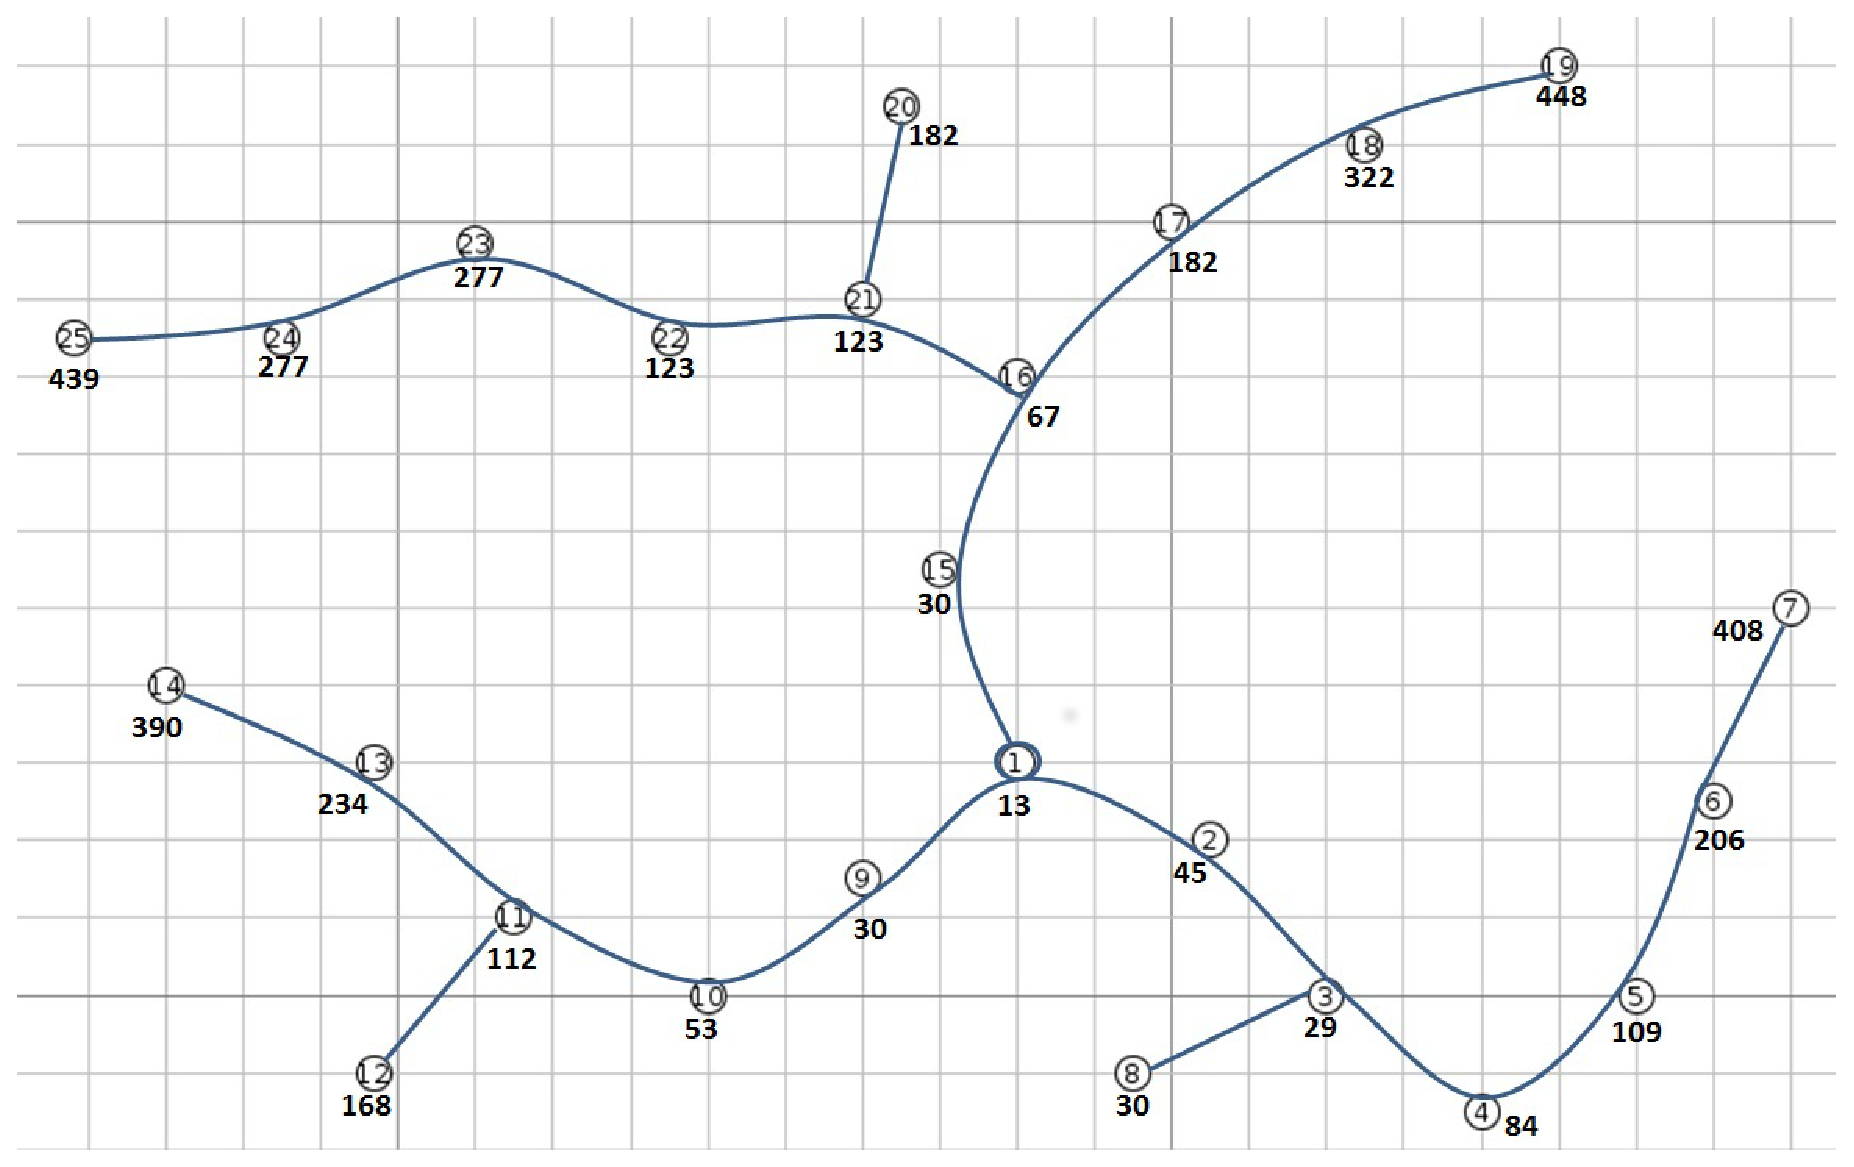
\includegraphics[width=\linewidth]{Tree}
    }    
        \caption{IWS and Relative position of nodes}
    \label{fig:elliptopo} 
\end{figure} 
Figure~\ref{fig:elliptopo} shows the relative positions of the motes with mote ID written at the centre of the tiny circle and IWS beneath the circle---the IWS has been calculated using  the utility function shown in Equation~\ref{eqn2}.
Each of the motes were considered as intrusion point in the process of measuring the IWS.
The IWS increases linearly with the increase in distance from the sink.
The `distance' term can be misleading without further clarification.
Euclidean distance between a mote and the sink does not make useful sense as the packets in the network must travel using a relay mechanism through other motes in the network.
Because of the availability of the multiple paths, it is not possible to quantify the exact distance that a packet would travel while transporting from a mote to the sink.
However, an estimation of distance along the most probable link path based on the connectivity may be considered.



\begin{figure}[bh!]
	\centering
	\resizebox{\linewidth}{!}{
        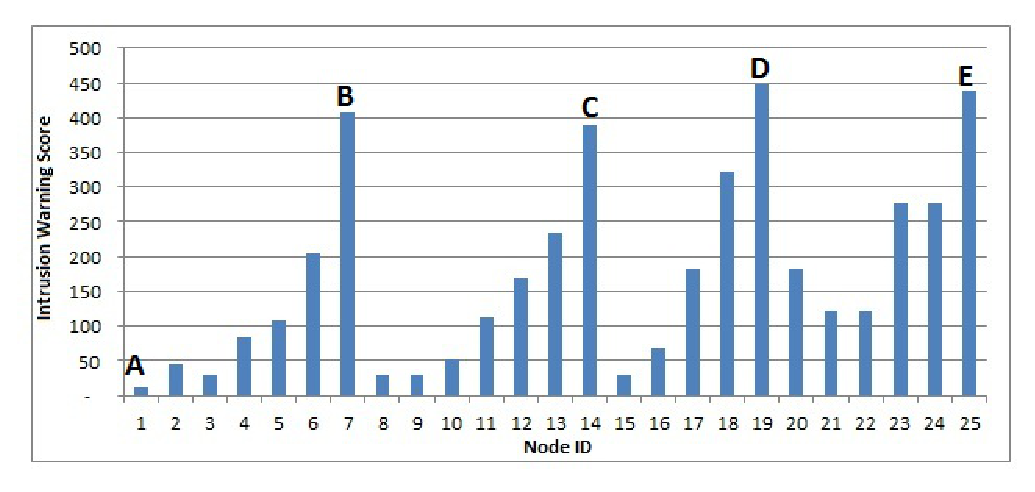
\includegraphics[width=\linewidth]{Tree_column}
    }
     \caption{Comparison of IWS at different motes}
     \label{fig:ellipgraph}
\end{figure}

The IWS is considerably higher for intrusion at distant motes than those that are close to the sink.
This phenomena is topology dependent, which also implies  that it is connectivity dependent.
It is possible that if the IWS distribution in a network is organised in a specific order, it would represent the original topology in some fashion.
For example, in the tree topology, the major branches are represented by linear rising slope in Figure~\ref{fig:ellipgraph}.
The branch along node ID 1 to 7 can be imagined as a line from point `A' to `B'. Similarly, distant point of other branches can also be imagined at points `C',`D', and`E'.

%IWS at different motes differ considerably: the motes close to the sink have very low IWS in comparison to the distant motes.
%The observation is also evident from Figure~\ref{fig:ellipgraph}.
% <dme> covered indirectly in the paragraphs below, I think.

The main contribution of this research comes from the ability to report an anomaly using a quantitative term such as the IWS.
For example:  a regular legitimate update, initiated from node ID 1, resulted in an IWS of 13.
The result matched the theoretical expectation of a very low IWS.
In addition to this, when intrusion scenarios were simulated from the nodes near the sink, the IWS reported was fairly low, e.g. 30 for mote ID 3, 8, 9, and 15
 and 45 for node 2. 
Because of the fact that the IWS of the motes close to the sink are likely to be very low---which is inline with the theoretical expectation---it is quite difficult to conclude if such an IWS indicates an intrusion. 
However, for the distant motes, the IWS is quite high and the IDS can conclude that such cases are intrusions, e.g.\ an IWS of 408 for mote ID 7, 390 for mote ID 14, and 322 for mote ID 18.
%277 for mote ID 23
%and likewise indicate intrusion.


While reporting severity or likelihood of an intrusion in quantitative terms like the IWS is useful itself, the IDS can also detect the source of intrusion and its extent. 
The IDS analyses update timing of all motes to identify the source of intrusion. 
For example, Table~\ref{tab:tree_time_18} presents the update time recorded at different motes when an intrusion was initiated from note 18.
The timing data shows that the lowest timing was recorded at node 17 and 19 which was equal to 15 seconds.
Node 18 is not expected to report any time because of three practical reasons: 
%<Ash> I am not comfortable with this arguments anow because of the way we've changed the assumptions now. Well, I'll revisit the assumptions again and then come back here later.
\begin{inparaenum}
\item node 18 initiated the update, so it was updated at $0$ seconds;
\item it acted as a sink, according to the protocol it did not require notifying its update time to any other mote; and 
\item it is the compromised node whose protocol is expected to be altered.
\end{inparaenum}
From this information, the IDS can conclude that node 18 was the intrusion point.
The extent of intrusion, as specified earlier, is found out from reported version information.

\begin{table*}[t!]
\centering
\begin{tabular}{|l|*{17}{r|}r|}
\hline
\bd{Node ID}           & \bd{4} & \bd{7} & \bd{8} & \bd{9} & \bd{10} & \bd{11} & \bd{12} & \bd{14} & \bd{15} & \bd{16} & \bd{17} & \bd{19} & \bd{20} & \bd{21} & \bd{22} & \bd{23} & \bd{24} & \bd{25}\\
%Mote ID           & 1 & 2 & 3 & 4 & 5  & 6 & 7 & 8 & 9 & 10 & 11 & 12 & 13 & 14 & 15  & 16 & 17 & 18 & 19 & 20 \\
\hline
\bd{Update Time}  &   277 	&  400 	& 231 	& 211 	& 231 &	 287 	& 318 &	 311 &	 139 & 72 &	 15 &	 15 &	 84 	& 72 	& 139 &	 185 &	185 & 273 \\
\hline
\end{tabular}
\caption{Update Time of motes when intrusion was initiated from node 18. Data from node 1, 2, 3, 5, 6 and 13 omitted due to space limitation.}
\label{tab:tree_time_18}
\end{table*}

%Identifying node failure and node compromise
% In addition detecting intrusion related information, the IWS is also able to detect node failures in the WSN.
% The case of a node not reporting its update time within a specified delay is handled by an error recovery procedure put in place by the IDS.
% If the recovery procedure fails, the node is considered to have failed or have been compromised.
% A unusual update time chronology and resulting unusual IWS  indicates the probability of some other types of attacks like node relocation, node repudiation, node compromise, not just a transient failure which is something worth paying attention to.
% <dme> It's a pretty inefficient way to detect problems, and no evaluation is given, so I've dropped this text.
% However, such failure resulting into contribution towards an IWS which is quite different for the update pattern detected from the timing information reported by the other nodes.
% The IDS structure is such that it has an expected pattern and shape of IWS for an intrusion at some specific point.
% If the shape is distorted to a great extent, it indicates some unusualness which can be attributed to some other phenomena like node failure or compromise.
% The node failure or node compromise can take place concurrently with or without intrusion.
% It might also indicate a different type of attack associated with a physical intrusion.
% An interpretation form the IDS view of the topology would enable identification of some other types of attacks in WSN like node relocation, node repudiation, node compromise.
% \notedme(1){This paragraph probably needs to be much shorter. The point is simply that you're looking for a timing pattern, and that it involves a fair few transmissions. Thus if you see an anomaly, given that you're already comparing against a statistical distribution, it's probably not just a transient failure, and thus something worth paying attention to.}
%%<Ashraf> addressed


\section{Conclusion}
\label{sec:concl}

Collaboration between wireless sensors and robotics can offer great advantages. 
With adoption of collaborative robotics increasing rapidly, the security of the environment in sensor assisted navigation or inter-robot communication over wireless media is of great importance.
Supporting a group of robots with WSNs  can extend the capability of both. 
%Sensors can sense, they cannot react. 
%Sensors have huge limitations in their capability to be in dependently useful. 
% <dme> above isn't necessarily true; weak text / points.
Sensors are not suitable for heavy computational tasks because of constraints on power, memory, and storage. 
On the other hand, robots have greater capabilities like mobility, performing resource intensive tasks, and operating in unfavourable
environments.
Combining the capabilities of WSN and robots is appealing. 
% However, sensors need to address its limitations for the technology to be effectively useful for robotics. 
% <dme> weak text - not specific enough.


In this paper, we modelled an IDS solution to intrusion in WSN software update protocols.
We discussed the potential dangers that are associated with WSN OTA software updates.
While OTA update protocols make certain WSN management tasks easy, they also remain vulnerable to intrusion attempts.
%An adversary can take advantage of the resource constrained nature of the sensor motes and employ enough resources to break in through the limited protection the sensors are armed with.
% <dme> don't believe this
To help manage this problem, we have suggested a passive security mechanism---an IDS.
A robot can also host the IDS in a collaborative environment.
The IDS is generally housed in a server that remains physically connected to the  sink. 
The system watches over the timing of software update patterns using a modified version of the Deluge protocol.
Whenever a mote is updated, it sends update-related information to a designated sink using a datagram.  
Related information from the datagram is filtered by the ITC for further processing at the IDS.

The first contribution of this research is quantifying intrusion probability through a quantitative IWS metric. 
%The IWS is a quantitative indicator of possible intrusion.
The utility function that computes the IWS is designed to neutralise the undesired %/unexpected
changes in mean and standard deviation which are expected to contribute to a near zero IWS.%\notedme{unclear}

The other important contribution is related to identifying the location and extent of intrusion.
The IDS can indicate the approximate location from where the intrusion was initiated by analysing timing data.
It can also decide on the extent of intrusion based on reported software version information.
%Besides, the IDS also can indicate some other kinds of anomalies such as node relocation, node repudiation, node compromise and so on.

While identifying intrusions in OTA software updates is a difficult task, under certain conditions it is practical.
% removing the effects is quite easy.
%Unless an intrusion leads to a DoS attack, the intrusion effect can be easily removed by initiating another update of the legitimate software from the sink.
% <dme> it's too risky to say something that sounds so wrong if readers might not have seen the part that says sections of the WSN OS don't get updaded.
There are still other potential security problems to investigate, of course. For example, protection against DoS attacks in which the use of the network is lost and needs major effort to recover, is beyond the scope of this paper.

The IDS we described here has several limitations. 
It assumes some special cases like a static WSN with a single sink.
It also assumes that network-wide information will not be forged. %to have network wide transparent knowledge.
These assumptions may not hold in a real WSN.
%In addition to this, assumptions about the attacker are:
%the attacker can employ enough resources to break in the cryptographic protections in sensors; however, he is not able to modify the protocols in an uncompromised sensor.
% <dme> not correct
The IDS has an obvious functional limitation.
It cannot identify an intrusion in certain scenarios.
For example, when an intrusion takes place in close vicinity of the sink, theIWS may not always be sufficiently large to be identified as an intrusion.
Another limitation stems from the fact that the results are based on simulated data and needs support from real world implementation.
In future,  the IDS will be implemented and deployed to examine real-world performance including cases of multiple sinks and mobile sensors.


\bibliographystyle{IEEEtran}
\bibliography{icara}


% that's all folks
\end{document}



%  LocalWords:  Ashraful Alam dme uncompromised

